%%Designed for IEEE Transactions on Vehicular Technology, based on bare_jrnl.tex by Michael Shell.
%%December. 2015
%%Length Requirements: The complete manuscript  should be prepared in final IEEE typesetting with maximum page length limited to 15 pages for a Regular Paper and 5 pages  for a Correspondence. 
%%Contact Info: admin-tvt@ece.ufl.edu
%%Designed by TVT editorial office


\documentclass[journal,10pt]{IEEEtran}
\usepackage[T1]{fontenc}
\usepackage[latin9]{inputenc}
\usepackage{textcomp}
\usepackage{amsmath}
\usepackage{amssymb}
\usepackage{graphicx}
\usepackage{xcolor}

\begin{document}

\title{Simpler Multipath Detection for Vehicular OFDM Channel Tracking}

\author{Diego M\'endez-Romero, M. Julia Fern\'andez-Getino Garc\'ia,~\IEEEmembership{Member,~IEEE}

\thanks{Copyright (c) 2018 IEEE. Personal use of this material is permitted. However, permission to use this material for any other purposes must be obtained from the IEEE by sending a request to pubs-permissions@ieee.org.}

\thanks{The authors are with the Department of Signal Theory and Communica-
tions, Universidad Carlos III de Madrid (Spain). E-mail: \{dmendez, mjulia\}@tsc.uc3m.es.}}% <-this % stops a space
%\thanks{Manuscript received XXX, XX, 2015; revised XXX, XX, 2015.}

\markboth{IEEE Transactions on Vehicular Technology,~Vol.~XX, No.~XX, XXX~2018}
{}
%{Shell \MakeLowercase{\textit{et al.}}: Bare Demo of IEEEtran.cls for Journals}

\maketitle

\begin{abstract}
The ever increasing requirements in
wireless communications have led to the search for unexploited correlations
which could improve channel estimation and tracking. Kalman filtering
(KF) has been proposed to exploit several such correlations, e. g.
the time correlation in each tap in a multipath channel. When making full use of this correlation, however, a capital disadvantage of KF is its weak
performance in the face of a significant, occasional non-linearity,
such as the potential birth of a new tap in a multipath channel or
an active tap's death. These non-linearities are typical for vehicular applications. So far, solutions proposed to this birth-death
nonlinearity problem have been shown to be computationally prohibitive.
In this work, a simplified detection framework is introduced and a
computationally inexpensive Simplified Maximum a Posteriori (SMAP) estimator is derived. Under low to medium
SNR conditions, simulations show the channel tracking error can be
approximately halved (vs. simple KF) by this novel estimator in Orthogonal Frequency
Division Multiplexing (OFDM) systems.
\end{abstract}


\begin{IEEEkeywords}
OFDM, Kalman Filtering, vehicular, high-mobility, path birth-death, channel estimation.
\end{IEEEkeywords}


\IEEEpeerreviewmaketitle



\section{Introduction}

Orthogonal Frequency-Division Multiplexing (OFDM) has spread quickly
and it has become the base for many communication technologies, such as present-day Long-Term Evolution (LTE) systems. Recently, OFDM has also been proposed for providing broadband data services in high-mobility applications \cite{SHE17} such as high-speed rail \cite{GUO17}. Moreover, OFDM, in combination with other techniques such as filtering or spreading, is envisaged as the base for future waveforms in 5G scenarios.

In some OFDM environments, particularly in vehicular applications, it is necessary to track time-variant channels. For that purpose, one of the most frequently proposed techniques is
Kalman filtering (KF) and its many adaptions and extensions \cite{GRE01}.

Sometimes, some other information related to the channel is used to increase efficiency. In \cite{JEL17}, for example, KF is used in combination with structure information of the channel impulse response (CIR) to estimate OFDM channels in a sparsity-aware mode. Forward-backward and forward KF are used in \cite{ALN07} in combination with data restriction information to greatly enhance estimation in a recursive manner; however, at a very large computional cost. The combination of KF, sparsity exploitation and recursion has also been recently proposed in \cite{GUN17} for OFDM estimation. Other published proposals include the use of an Extended Kalman Filter for MIMO-OFDM \cite{DAL17}, a mixture KF for blind OFDM channel estimation \cite{ZHA04}, data-aided KF channel tracking \cite{8} and the combination of pilots and KF \cite{10}, to name but just a few.

KF's advantage is its optimality as an estimator for linear problems;
thus, if channel tracking can be approximated as a linear problem,
the KF solution is near-optimal. However, as requirements grow and
mobile communications spread into more dynamic channels, such as those of high-speed
railways \cite{12} in rugged terrain \cite{13} or Unmanned Aerial Vehicles (UAVs) \cite{14} in suburban/hilly terrain environments \cite{MAT16}, random intermittent multipath components (MPCs) appear. The corresponding non-linearities,
such as path birth and path death \cite{MAH17}, could be catastrophic for KF-based
estimation techniques. Accordingly, more powerful tap tracking techniques
will be needed in the future.

Few in-depth analysis for the non-linear tracking problem have been
published. So far, to our best knowledge, the only consistent proposal
for tap tracking under birth-death conditions has been to use Random
Set Theory (RST) models. In \cite{4,5}, three possible RST-based
estimators were compared; the so-called GMAP-III, which was proven
to be the best performer by far, comes at a computationally prohibitive
cost which renders it impracticable in real-world conditions. In this
paper, a simpler birth-death detection paradigm is introduced which,
in combination with KF, makes it feasible (i.e. computationally inexpensive)
to approximately halve channel tracking error vs. bare KF under low to medium
SNR conditions. This novel estimator is denoted Simplified Maximum
a Posteriori (SMAP) estimator.

This paper is organized as follows. In Section {\scshape ii}, the problem is formally
stated. Then, a quick review of approaches to channel tracking and
how to measure their quality is made in Section {\scshape iii}. The proposed SMAP
estimator is introduced in Section {\scshape iv}, and its simulated results are
shown in Section {\scshape v}. Finally, conclusions are extracted in Section
{\scshape vi}.

\section{Statement of the problem}

We consider an OFDM system employing $N$ orthogonal subcarriers,
transmitting OFDM symbols with a time duration $T_{symb}$ and a sampling
interval $T_{samp}$. It is assumed there is no out-of-band interference. Periodically, each subcarrier is used first for pilot symbols enabling channel estimation, and then for data transmission (through data blocks of fixed length $M_{inf}$). Each data block is preceded by $K$ pilot symbols, so
that the first $K$ sent symbols are pilot symbols used to estimate
the channel (by averaging over $K$); this channel estimation will be
considered ``valid'' and will be used for the whole subsequent $M_{inf}$-symbol data block transmission. Channel changes will be tracked only once every estimation period $T_{est}=(K+M_{inf})\cdot T_{symb}$, since a certain channel stationarity within each estimation period can be
assumed due to its coherence time and, accordingly, channel changes
can be reasonably modeled as occurring at the beginning of each estimation period.

If $k=\{1,...,K\}$ is the pilot symbol index in the $p$th estimation
period, then the received signal, which is the input for channel estimation,
can be given in vector form as:
\begin{equation}
\mathbf{y}_{p,k}=\mathbf{D}_{p,k}\mathbf{F}_{p}\mathbf{h}_{p}+\mathbf{z}_{p,k}
\end{equation}
where $\mathbf{y}_{p,k}=[y_{p,1,k},...,y_{p,N,k}]^{T}$, each $y_{p,n,k}$
(for $n=\{1,...,N\}$) represents the $n$th subcarrier observation
sample at time $t_{p,k}=(p-1)\cdot T_{est}+(k-1)\cdot T_{symb}$;
$\mathbf{D}_{p,k}=diag(d_{p,1,k},...,d_{p,N,k}),$with $d_{p,n,k}$
the training data on the $n$th pilot subcarrier at time $t_{p,k}$;
$\mathbf{z}_{p,k}=[z_{p,1,k},...,z_{p,N,k}]$, with $z_{p,n,k}$ representing
the zero-mean complex Gaussian additive noise having variance $\sigma_{z}^{2}$;
if $l=\{1,...,L(pT_{est})\}$ and $L(pT_{est})$ is the number of
active paths, then $\mathbf{h}_{p}=[h_{1}(pT_{est}),...,h_{L(pT_{est})}(pT_{est})]^{T}$,
with $h_{l}(pT_{est})$ the complex gain of the $l$th path at time
$p$, which, as previously explained, will be assumed constant for
the duration of the estimation period; and
\begin{equation}
\{\mathbf{F}_{p}\}_{n,l}=e^{-j2\pi n\cdot\frac{\tau_{l}(pT_{est})}{NT_{samp}}}
\end{equation}
where $\tau_{l}(pT_{est})$ is the delay of the $l$th path during
the $p$th interval. 

Clearly, since each data block is preceded by $K$ pilot symbols,
the received signal including reception of all $K$ pilot symbols
will be the matrix $\mathbf{Y}_{p}=[\mathbf{y}_{p,1},...,\mathbf{y}_{p,K}]$.
A guard time, named cyclic prefix, $T_{CP}$ is reserved between OFDM
symbol transmissions, so that $T_{symb}=NT_{samp}+T_{CP}$. It is
assumed that the multipath delay spread is smaller than $T_{CP}$.

Moreover, the active path gains are assumed to follow an underlying
Linear Gauss-Markov (LGM) model \cite{GRE01}. For ease of notation, $a_{p}^{(l)}=h_{l}(pT_{est})$ will
represent the $l$th path gain at time $p$. Provided that the $l$th path
is active and remains so, the probability density function (pdf) for $a_{p}^{(l)}$
would be given by both following equations:
\begin{equation}
f(a_{1}^{(l)})=N(a_{1}^{(l)};0,\sigma_{h_{l}}^{2})\label{eq:GML1}
\end{equation}
\begin{equation}
f(a_{p}^{(l)}|a_{p-1}^{(l)})=N(a_{p}^{(l)};\lambda a_{p-1}^{(l)},(1-\lambda^{2})\sigma_{h_{l}}^{2})\label{eq:GML2}
\end{equation}
where $\sigma_{h_{l}}^{2}$ is the average energy of the $l$th path
and $\lambda$ is the temporal self-correlation of each active path
gain. However, notice that, if the $l$th path is not active (because
it has ``died''), then $h_{l}(pT_{est})$=0, i.e. path gain equals
zero. Each active path has a probability $P_{death}$ of becoming
inactive; each inactive path has a probability $P_{birth}$ of becoming
active.

The problem under consideration can now be formulated as follows:
given the observations (1), determine a computationally inexpensive
causal estimator $\hat{\mathbf{h}}_{p}$ for $\mathbf{h}_{p}$, relying
upon $\{\mathbf{Y}_{1:p}\}$. Since ``computationally inexpensive''
may be too vague a term, a slightly different, more precise formulation
of the problem would be: determine the $simplest$ causal estimator
for $\mathbf{h}_{p}$ exploiting path self-correlation to the extent
of getting $most$ of the theoretically maximum possible reduction
in Channel Tracking Mean Squared Error (CTMSE), defined as:
\begin{equation}
CTMSE\,\triangleq||\sum_{p}\hat{\mathbf{h}}_{p}-\mathbf{h}_{p}||_{2}^{2}\label{eq:CTMSE}
\end{equation}
where $||\cdot||_{2}$ denotes the Euclidean norm.

\section{Channel tracking}

\subsection{Linear Gauss-Markov (LGM) models}

Let us consider a LGM model where all paths are active and they follow
(\ref{eq:GML1}) and (\ref{eq:GML2}). These LGM models have been
previously used in the literature (e.g. in \cite{4,5}) and they make
it possible to derive a computationally inexpensive, optimal estimation
through Kalman filtering. However, they are ideal channels whose behaviour
may or may not approximate specific real channels. In this regard,
a severe disadvantage is that, since they are perfectly linear, they
don't allow for jumps.

\subsection{KF-based approaches}

Under a LGM model, a KF-based approach can be easily implemented.
Kalman filtering is an algorithm weighting optimally two information
sources: a theoretical one (in our case, the LGM channel model) and
another one based on noisy measurements. The Least-Squares (LS) channel
estimation, $\hat{\mathbf{a}}_{p}^{LS}$, can be interpreted as a
noisy measurement of the true channel $\mathbf{a}_{p}=[a_{p}^{(1)},...,a_{p}^{(L)}]^{T}$:
\begin{equation}
\mathbf{u}_{p}\triangleq\hat{\mathbf{a}}_{p}^{LS}=\mathbf{a}_{p}+\mathbf{v}_{p}\label{eq:noisyMeasu}
\end{equation}
where $\mathbf{v}_{p}=[v_{p}^{(1)},...,v_{p}^{(L)}]^{T}$ is the measurement
noise and $\mathbf{u}_{p}=[u_{p}^{(1)},...,u_{p}^{(L)}]^{T}$ will
be used for ease of notation. Since path independence is being assumed,
this translates into $L$ scalar equations. Thus, a bank of independent
Kalman filters could be used to track the whole channel, whereby each
Kalman filter would receive the LS-estimated tap gain and would compute
the corresponding KF tap estimation, $\hat{u}_{p}^{(l)}(+)$, and also the expected path gain
at time $p+1$, the so-called Kalman prediction, $\hat{u}_{p+1}^{(l)}(-)$. Please note that the $(-)$ sign denotes prediction while $(+)$ denotes estimation. This distinction is important (algorithms are different) and relevant to this paper.

This KF approach is optimal when non-linearities are absent. However,
the disappearance and reapparance of paths (i.e. the real channel
``jumping'' in a way the perfect LGM model cannot fit) introduce
a severe nonlinear distortion and KF performance degrades catastrophically.

\subsection{RST-based approaches}

RST-based approaches have proven that, under birth-death conditions,
a very good estimator is the so-called GMAP-III, which essentially
adds a death-birth detector before the KF step. Thus, you first detect
which paths are active, and then you estimate active paths' gains.
The GMAP-III estimator was proposed in \cite{4} with the following
definition:
\begin{equation}
\textrm{GMAP-III}:\begin{cases}
\widehat{\pi(\mathcal{H}_{p})}=\textrm{arg max\ensuremath{_{\pi(\mathcal{H}_{p})}f_{\pi(\mathcal{H}_{p})|\mathcal{Y}_{1:p}}(\pi(\mathcal{H}_{p})|\mathcal{Y}_{1:p})\textrm{,}}}\\
\widetilde{\mathbf{h}}_{p}=\int_{\mathbb{R^{\textrm{2\ensuremath{|\widehat{\pi(\mathcal{H}_{p})}|}}}}}\mathbf{h}_{p}f_{\mathbf{h}_{p}|\mathcal{Y}_{1:p}}(\mathbf{h}_{p}|\mathcal{Y}_{1:p})d\mathbf{h}_{p}
\end{cases}\label{eq:GMAP-III}
\end{equation}
where $f(\cdot)$ represents a pdf and
\begin{equation}
f_{\pi(\mathcal{H}_{p})|\mathcal{Y}_{1:p}}(\pi(\mathcal{H}_{p})|\mathcal{Y}_{1:p})=\int_{\pi'(\mathcal{H}_{p})}f(\mathcal{H}_{p}|\mathcal{Y}_{1:p})\delta\mathcal{H}_{p}
\end{equation}

(For further details on notation, see \cite{4}). However, death-birth detection
under the RST framework can be difficult to handle and computationally
prohibitive, e.g. in \cite{4}, death-birth detection is done through
a 10,000-particle filter that approximates (\ref{eq:GMAP-III}).
It is evident that a much simpler, suboptimal estimator is required for practical applications. Such an estimator
will be proposed in Section {\scshape iv}, but, firstly, a measurement of its
quality will be introduced in the following Section.

\subsection{Measuring the quality of simpler estimators}

Our objective is to reduce CTMSE as defined in (\ref{eq:CTMSE}).
What is the theoretically maximum possible reduction in CTMSE when
using some given birth-death information?

First, let us consider Fig. 1 to see how path birth-death information
could be used in practice. Following the notation for (\ref{eq:noisyMeasu}),
Fig. 1 starts with the LS channel estimation, $\hat{\mathbf{a}}_{p}^{LS}$,
having its individual path components extracted and fed into individual
path birth-death detectors. These detectors are like switches and
are represented as such in Fig. 1: on birth detection, the $l$th
LS path estimation is fed into the $l$th KF, which starts tracking and provides $\hat{u}_{p}^{(l)}(+)$, the $l$th estimated path gain (not to be confused with $\hat{u}_{p}^{(l)}(-)$, which is a prediction done at time $p-1$);
on death detection, however, the $l$th estimated path gain is put
to zero until the next time the $l$th path is detected to be reborn.
Since the problems of birth-death detection, on the one hand, and
active-path tracking, on the other hand, are separable in nature,
the maximum reduction in CTMSE is obtained when, for each path, an
optimal birth-death detector is connected to a KF.

\begin{figure}
\includegraphics[scale=0.10]{Fig_1}

\caption{Tap birth/death detectors and KF bank arrangement.}

\end{figure}

Now, let us suppose perfect information on the active/inactive status
of each tap was available. What would the theoretically maximum possible
reduction in CTMSE be when using this perfect birth-death information?
Death-birth detectors would then be always right, and looking into
this ideal case, henceforth the Ideal Switching System (ISS), could
provide useful information about the problem and the quality of different
solutions to it.

Thus, the ISS is the system drawn in Figure 1 when death/birth detectors
detect 100\% of births and 100\% of deaths, with no false birth/death
detection. It is also possible to easily define an x\%-degraded Ideal
Switching System (IIS-x\%), which is a switching system detecting
x\% of births and x\% of deaths, with no false birth/death detection.
These degraded ISS were simulated for the problem at hand (for more
details, see Section {\scshape v}) and Table 1 shows the \% reduction (vs. the
LS method, i.e., no KF) these near-optimal ISS devices could achieve,
as measured in CTMSE, for different SNR values. A quick look at Table
1 makes it possible to conclude that ISS performance in terms of CTMSE
degrades significantly even with minor reductions in the \% of birth/death
detections. For higher SNR, the degradation is so catastrophic that
the conventional LS estimation performs better than a slightly degraded
ISS (e.g. an ISS-99\%, negative value in the bottom-right corner of
Table 1). Do note, however, that the degraded ISS greatly improves
estimation over conventional LS estimation for low-to-medium SNR levels.

These conclusions are also backed by Figure 2, which plots the degraded
systems' performance in terms of CTMSE. This kind of plots let us
establish a natural measure for an estimator's fitness in the context
of the previously defined problem. Some estimator could be, for example,
better than ISS-97\% and worse than ISS-98\%, meaning that it would
be slightly better than a degraded ISS where detectors detected 97\%
of births and 97\% of deaths, but not as good as a system detecting
98\% of both.

It must also be noted that the performance of OFDM is sensitive to the 
existence of carrier frequency offset (CFO). However, there are numerous 
proposals in the literature for frequency synchronization in OFDM, based 
on specific headers or pilot sequences, which attain an adequate 
synchronization with negligible residual errors (refer to recent works \cite{ZHA17, MUK16, ZHA18}).

\begin{table}
\centering{}\caption{\% reduction in CTMSE for differently degraded ISS vs. LS estimation.}
\begin{tabular}{|c|c|c|c|c|}
\hline 
SNR {[}dB{]} & ISS & ISS-99.9\% & ISS-99.5\% & ISS-99\%\tabularnewline
\hline 
\hline 
8.5 & 72.84 & 72.46 & 69.35 & 66.52\tabularnewline
\hline 
11 & 70.16 & 68.86 & 64.81 & 59.14\tabularnewline
\hline 
13.5 & 65.40 & 63.75 & 56.81 & 45.77\tabularnewline
\hline 
16 & 56.93 & 53.83 & 40.59 & 23.77\tabularnewline
\hline 
18.5 & 41.81 & 35.29 & 8.72 & -16.40\tabularnewline
\hline 
\end{tabular}
\end{table}

\begin{figure}
\includegraphics[scale=0.62]{Fig_2}

\caption{Average CTMSE performance of LS vs. ISS and different x\%-degraded ISS}

\end{figure}

\section{Proposed scheme: SMAP estimator}

A Bayesian-inspired estimator of $\mathbf{h}_{p}$ can be defined
by using KF in combination with the three following heuristics for
path birth-death detection: 1) detect death if the path gain jumps
into approx. zero; 2) detect death if the path gain has slowly converged
into approx. zero; 3) detect birth if the path gain is far from zero.
These three rules can ultimately be simplified to three threshold comparisons, as shown in the three following Sections through simple theoretical derivations. The specific threshold parameter values can then be obtained empirically through precision simulations, as discussed and shown in Section {\scshape iv.d}. 

\subsection{Memoryless detection of large leaps into a narrow, zero-centered
range}

When the $l$th path is dead, its true gain is, by definition, zero.
Thus, the observed gain is just the (Gaussian) noise. Hence, path
gain measurement $u_{p}^{(l)}$ follows a Gaussian distribution:
\begin{equation}
u_{p}^{(l)}|l\,is\,dead\sim N(0,\sigma_{v^{(l)}}^{2})
\end{equation}
where $\sigma_{v^{(l)}}^{2}$ is the variance of path (measurement)
noise $v_{p}^{(l)}$. On the other hand, if $l$th path is active,
then its gain follows a Gaussian centered on the previously expected
gain, $\hat{u}_{p}^{(l)}(-)$, the Kalman prediction computed at time
$p-1$ (this is a feature of KF). Two variance sources can be identified for this Kalman prediction: measurement noise $\sigma_{v^{(l)}}^{2}$ and channel tap variance $(1-\lambda^2)\sigma_{h}^2$. Thus, it is convenient to consider
\begin{equation}
u_{p}^{(l)}|l\,is\,alive\sim N(\hat{u}_{p}^{(l)}(-),\sigma_{A}^{2})
\end{equation}
where
\begin{equation}
\sigma_A=q_A\cdot\sqrt{\sigma_{v^{(l)}}^{2}+(1-\lambda^2)\sigma_{h}^2}
\end{equation}
and $q_A$ is an error-minimizing positive threshold (as later explained in Section {\scshape iv.d}).


Let us assume that the path was alive at time $p-1$. Then, either
path death happens at time $p$ (with prior probability $P_{death}$)
or the path will still be alive (with prior probability $1-P_{death}$).
Thus, a maximum a posteriori criterium leads to detecting ``death''
whenever
\begin{equation}
P_{death}\cdot f(u_{p}^{(l)}|l\,is\,dead)>f(u_{p}^{(l)}|l\,is\,alive)\cdot(1-P_{death})\label{eq:DeathDetector}
\end{equation}
where $f(\cdot)$ represents a pdf and the events ``$l$ is dead/alive'' mean that the $l$th path
is dead/alive, respectively. Note that this detector compares two
scaled Gaussian pdfs, so an equivalent expression to (\ref{eq:DeathDetector})
would be:
\begin{equation}
\begin{split}
P_{death}\cdot\frac{1}{\sqrt{2\pi}\sigma_{v^{(l)}}^{2}}\cdotp e^{-\frac{(u_{p}^{(l)})^{2}}{2\sigma_{v^{(l)}}^{2}}}>\frac{1}{\sqrt{2\pi}\sigma_{A}^{2}}\cdotp e^{-\frac{(u_{p}^{(l)}-\hat{u}_{p}^{(l)}(-))^{2}}{2\sigma_{A}^{2}}}\cdot \\ \cdot(1-P_{death})
\end{split}
\end{equation}

By taking logarithms and simple rearrangement, another equivalent expression can be found:
\begin{equation}
ln(\frac{P_{death}}{1-P_{death}})>\frac{(u_{p}^{(l)})^{2}}{2\sigma_{v^{(l)}}^{2}}-\frac{(u_{p}^{(l)}-\hat{u}_{p}^{(l)}(-))^{2}}{2\sigma_{A}^{2}}
\end{equation}
where $ln(\cdot)$ denotes the natural logarithm.

\subsection{Memory detection of a sequence at a close range of zero}

Let the $l$th path gain be active and close to zero (but never exactly
zero, since it is active!) at time $p$, i.e. $0\neq{u}_{p}^{(l)}\approx0$; since large leaps are highly improbable as Gaussian
outliers \cite{7}, let's assume that path gain will always stay close
to zero at time $p+1$. (This is a reasonable assumption if done only
for very short sequences, typically 2 or 3 succesive samples; it is in these short transitions where simple KF gets ``confused'' and needs most help). Thus,
the active path is assumed to be close to zero, continously active
and static, and the observed path gain is assumed to be just measurement
noise (a reasonable assumption when path gain is very close to zero).
Under these assumptions, the probability of having a sequence $\{|{u}_{p+1}^{(l)}|,...,|{u}_{p+s}^{(l)}|\}$ of length
$s$ at any range $q_{B}\cdot\sigma_{v}$ from zero, such that the
path is continously active and $\{|{u}_{p}^{(l)}|,...,|{u}_{p+s}^{(l)}|\}<q_{B}\cdot\sigma_{v}$,
is:
\begin{equation}
P_{seq\_in\_rge}=(1-P_{death})^{s}\cdot(1-2Q(q_{B}))^{s}\label{eq:Tunnel}
\end{equation}
where $Q(\cdotp)$ is the Q-function and $q_{B}$ is any arbitrary
threshold consistent with the aforementioned assumptions. Eq. (\ref{eq:Tunnel})
follows directly from the properties of the Gaussian distribution
\cite{7}. On the other hand, the probability of a path dying right
before the sequence or during the sequence (and not being reborn afterwards)
would be:
\begin{equation}
P_{dyi\_seq}=\sum_{i=0}^{s}(1-P_{death})^{i}\cdot P_{death}\cdot(1-P_{birth})^{s-i}
\end{equation}

Thus, if the system is continuously monitoring the presence of sequences
in this range, path death can be decided following a simplified maximum
a posteriori criterium whenever:
\begin{equation}
P_{dyi\_seq}>P_{seq\_in\_rge}\label{eq:MAP1}
\end{equation}

Thus, after setting a single appropiate threshold $q_{B}$ not too
far from zero and a short enough sequence length $s$, path death
can be decided trivially when an $(s+1)$-long sequence $\{|u_{p}^{(l)}|,...,|u_{p+s}^{(l)}|\}<q_{B}\cdot\sigma_{v}$
has been detected.

For example, if a sequence monitor for $q_{B}=\sigma_{v^{(l)}}^{2}/3$
and $s=2$ is set up, then this detector would decide ``dead'' after
a 3-long sequence $\{|u_{p}^{(l)}|,...,|u_{p+s}^{(l)}|\}<q_{B}\cdot\sigma_{v^{(l)}}=\sigma_{v^{(l)}}^{3}/3$
per (\ref{eq:MAP1}). Appendix {\scshape a} shows that, if assumptions are reasonable and hold true, the probability of having made the wrong decision is:
\begin{equation}
P_{err}=\frac{(1-P_{death})^{s}\cdot(1-2Q(q_{B}))^{s}}{P_{aux}+(1-P_{death})^{s}\cdot(1-2Q(q_{B}))^{s}}\label{eq:PError}
\end{equation}
where
\begin{equation}
P_{aux}=\sum_{i=0}^{s}(1-P_{death})^{i}\cdot P_{death}\cdot(1-P_{birth})^{s-i}
\end{equation}

\subsection{Birth detection}

Birth detection could easily be implemented as a threshold detector
that decides ``alive'' whenever $|u_{p}^{(l)}|>q_{C}\cdot\sigma_{v^{(l)}}$,
for a certain threshold $q_{C}$. Even if $P_{err}$ per (\ref{eq:PError})
were too high (close to 0.5), a very sensitive birth detector (a very
low $q_{C}$) would correct potential errors very early. Thus, detecting
a path birth is a correct decision not only when a new path is created,
but also when a path was wrongly detected as ``dead''.

Let's assume our birth detection happens immediately after having
decided ``path is dead'' in the scenario described in Section
{\scshape iv.b}. Since $P_{err}$ in (\ref{eq:PError}) is the probability
of that previous decision having been wrong, and since noise can make
an LS estimate of a dead path deviate outside a $q_{C}$ range from
zero with a probability $2Q(q_{C})$, then the probability of correcting
a previous error would be:
\begin{equation}
P_{corr}=P_{err}\cdot(1-P_{death})\cdot2Q(q_{C})
\end{equation}

On the other hand, a new path could have been created (with prob.
$P_{birth}$) if the previous decision (``dead path'') was right
(with prob. $1-P_{err}$). For simplicity purposes, let's assume that
newly created paths start at $|u_{p+1}^{(l)}|>q_{C}\cdot\sigma_{v^{(l)}}$.
Thus, the probability of correctly detecting a new birth would be:
\begin{equation}
P_{birth\thinspace det}=(1-P_{err})\cdot P_{birth}
\end{equation}

A birth decision would be wrong if the path was erroneously detected
as dead at time $p$ but it has recently become dead at time $p+1$
and noise puts it outside the detection limits, or when it was correctly
detected as dead at time $p$ and is still dead, but noise makes the
observation sample shoot outside the detection limits: 
\begin{equation}
P_{false\,det}=P_{err}\cdot P_{death}\cdot2Q(q_{C})+(1-P_{err})\cdot(1-P_{birth})\cdot2Q(q_{C})\label{eq:False_Det}
\end{equation}

Thus, a simplified maximum a posteriori criterium would decide ``birth''
whenever:
\begin{equation}
P_{corr}+P_{birth\,det}>P_{false\,det}
\end{equation}
These expressions look cumbersome but, in fact, you only need them
to obtain any appropiate $q_{C}$ for which (\ref{eq:False_Det})
holds true. Once a single appropiate threshold $q_{C}$ is set, path
birth can be decided trivially when $|u_{p}^{(l)}|>q_{C}\cdot\sigma_{v^{(l)}}$
has been detected. When birth is detected, the KF is restarted and
the first estimate is the LS estimate.

\subsection{Threshold parameter values}

The system resulting from the three detection heuristics shown above
and a connected KF block will be called ``Simplified Maximum a Posteriori''
(SMAP) estimator.

The proposed method, as suggested by the theoretical analysis in previous Sections, could have a positive performance independently from the specific choice of threshold values, provided that they reasonably fit the assumptions in Section {\scshape iv}.
Even though results (in Section {\scshape v}) will show the system to be rather robust to variations in parameter value selection, it is convenient to fine-tune it by obtaining an optimal set of parameter values for $q_{A}$, $q_{B}$ and $q_{C}$ through simulations. Several strategies are legitimate for this purpose. A set of values could be optimised in terms of MSE reduction, BER/SER reduction, or a combination of performance and sensitivity. In Section {\scshape v}, an approach based on MSE reduction is implemented and a sensitivity analysis is performed. Simulation results back the theoretical derivations and the optimization strategy advocated here.

\section{Simulation results}

A system with $N_p=3$ pilot subcarriers is considered, with $K=8$ pilot symbols per subcarrier before data transmission. The average energy per pilot symbol, $\sigma_{s}^{2}$, is uniform, and a BPSK modulation scheme is assumed. Channel assumptions include a uniform multipath delay profile, multipath spread smaller than the guard time, and uncorrelated path gains. The overall channel energy is normalized to one. OFDM symbols were transmitted through a channel with $L_{max}=3$, $P_{birth}=0.05$ and $P_{death}=0.05$. Threshold parameter values $q_A=0.23$, $q_B=0.30$ and $q_C=0.62$ were obtained through simulation-based MSE optimization for $s=1$ and form the basis for the simulation results shown here. Note that this prior optimization is always performed offline and, thus, it does not increase online computational complexity. This channel was then tracked for 200,000 estimations periods ($2\cdot10^5\cdot T_{est}$).
Individual paths were assumed to have the same average energy $\sigma_{h}^{2}$
over long periods and $\lambda=0.999$. This choice of parameters
makes it possible to compare the performance of the SMAP vs. the computationally
heavier methods outlined in \cite{4} and the KF system advocated
in \cite{10}.

Fig. 3 shows the performance (in terms of CTMSE, as per (\ref{eq:CTMSE}))
of our proposed SMAP estimation vs. a scenario with perfect information
(ISS), almost perfect information (ISS-99\%) and a KF system. It can
be seen that the SMAP estimator is very similar in performance to
ISS-99\%. This means the SMAP estimator gets most of the reduction
attainable by an ISS, but with a trivially low computational cost,
for low-to-medium SNR.

\begin{figure}
\begin{centering}
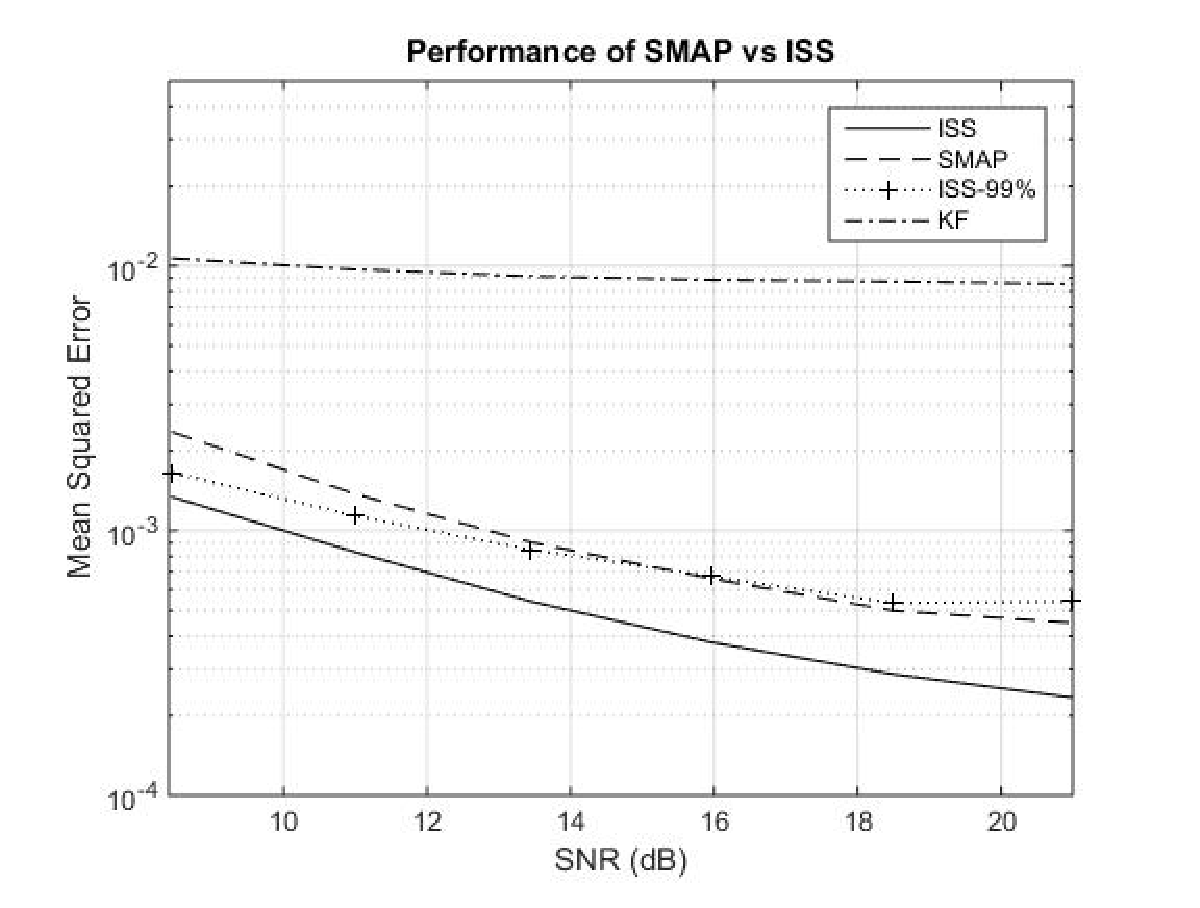
\includegraphics[scale=0.48]{Fig_3}
\par\end{centering}
\caption{Average CTMSE performance of proposed SMAP vs. ideal systems and KF}

\end{figure}

\begin{figure}
\begin{centering}
\includegraphics[scale=0.62]{Fig_4}
\par\end{centering}
\caption{Average CTMSE performance of SMAP with differently-deviated random thresholds vs. KF and optimal-threshold SMAP}
\label{fig:Sensi}
\end{figure}
A measurement of SMAP's robustness in the face of model uncertainty can be provided by setting random thresholds $q_A$, $q_B$ and $q_C$ extracted from Gaussians centered on the previously determined optimal values. Fig. \ref{fig:Sensi} shows simulation results for several standard deviation $\sigma$ values, e.g. $\sigma_\%=40\%$ means SMAP is not used now with optimal thresholds, but rather with several different random threshold triplets taken from Gaussians: $q_C\sim N(0.62,\sigma=0.62\cdot0.40=0.248)$, etc. In this particular simulation, 10 such random triplets were extracted for each $\sigma$ and SNR level. It is apparent from Fig. \ref{fig:Sensi} that large deviations result in smaller changes in CTMSE, especially when compared to bare Kalman. Thus, the use of a SMAP structure is shown to be a larger contributor to error reduction than the use of perfect thresholds in that SMAP structure. This low sensitivity to threshold deviations means SMAP is robust to some extent when facing some uncertainty in model parameters.
\begin{figure}
\begin{centering}
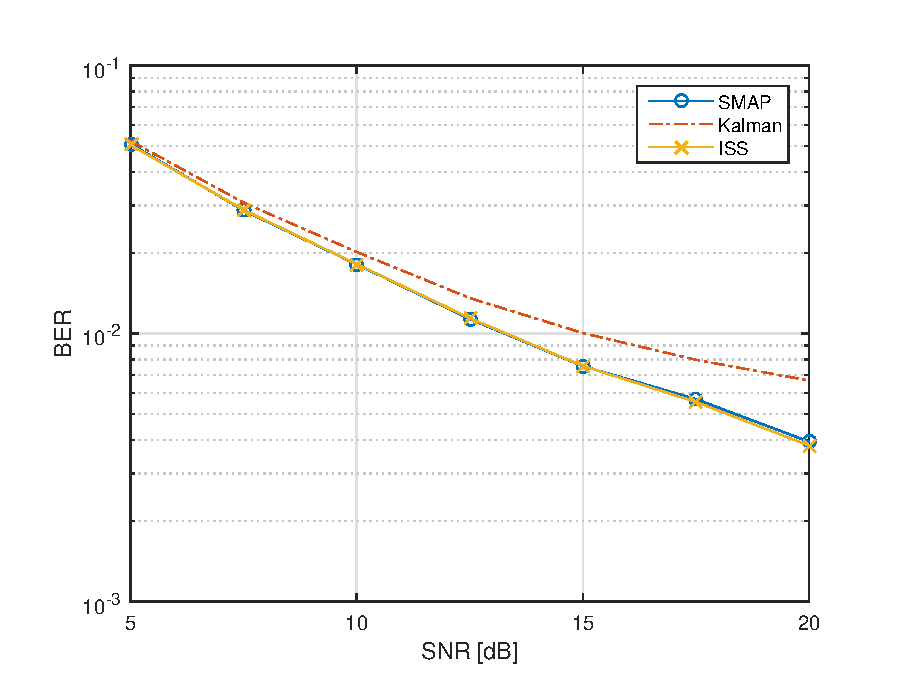
\includegraphics[scale=0.62]{Fig_5}
\par\end{centering}
\caption{BER performance of proposed SMAP vs. ideal system (ISS) and KF}
\label{fig:BER}
\end{figure}

Fig. \ref{fig:BER} shows the bit-error-rate (BER) performance of SMAP vs. the ideal system (ISS) and a KF system. This considers all samples when at least one path is active (channel energy at least 5\% of average channel energy), thus ignoring samples when all channel taps are zero and communication must be unfeasible. It must be noted that BER values were obtained without considering any channel coding scheme which would improve system performance. Results are unambiguous: the BER curve for SMAP matches the one for the ideal system (ISS) and both of them have a significant positive gap vs. bare KF.

Now let us take a closer look at Figs. 6-7, which show the estimated
path gain in SMAP and KF systems, respectively, for a signal-to-noise
ratio $\textrm{SNR}\triangleq\sigma_{s}^{2}/\sigma_{z}^{2}=15$ dB.
These figures support the thesis, already advanced in \cite{4}, that
a KF operating on $L_{max}$ paths suffers from a transient effect
from path death/birth. The proposed SMAP estimation adapts more quickly
to those non-linearities. This superior performance when a path disappears
or a new path is born can also be seen for $\textrm{SNR}=9$ dB in
Figs. 8-9 and for SNR = 21 dB in Figs. 10-11.

Moreover, this superior performance does not come at the expense of
a prohibitively high computational cost. On the contrary, each path
detector uses only the three computationally inexpensive threshold
comparisons outlined in Section {\scshape iv} to achieve an error reduction matching
that of a close-to-perfect path death/birth detection (ISS-99\%).

\begin{figure}
\begin{centering}
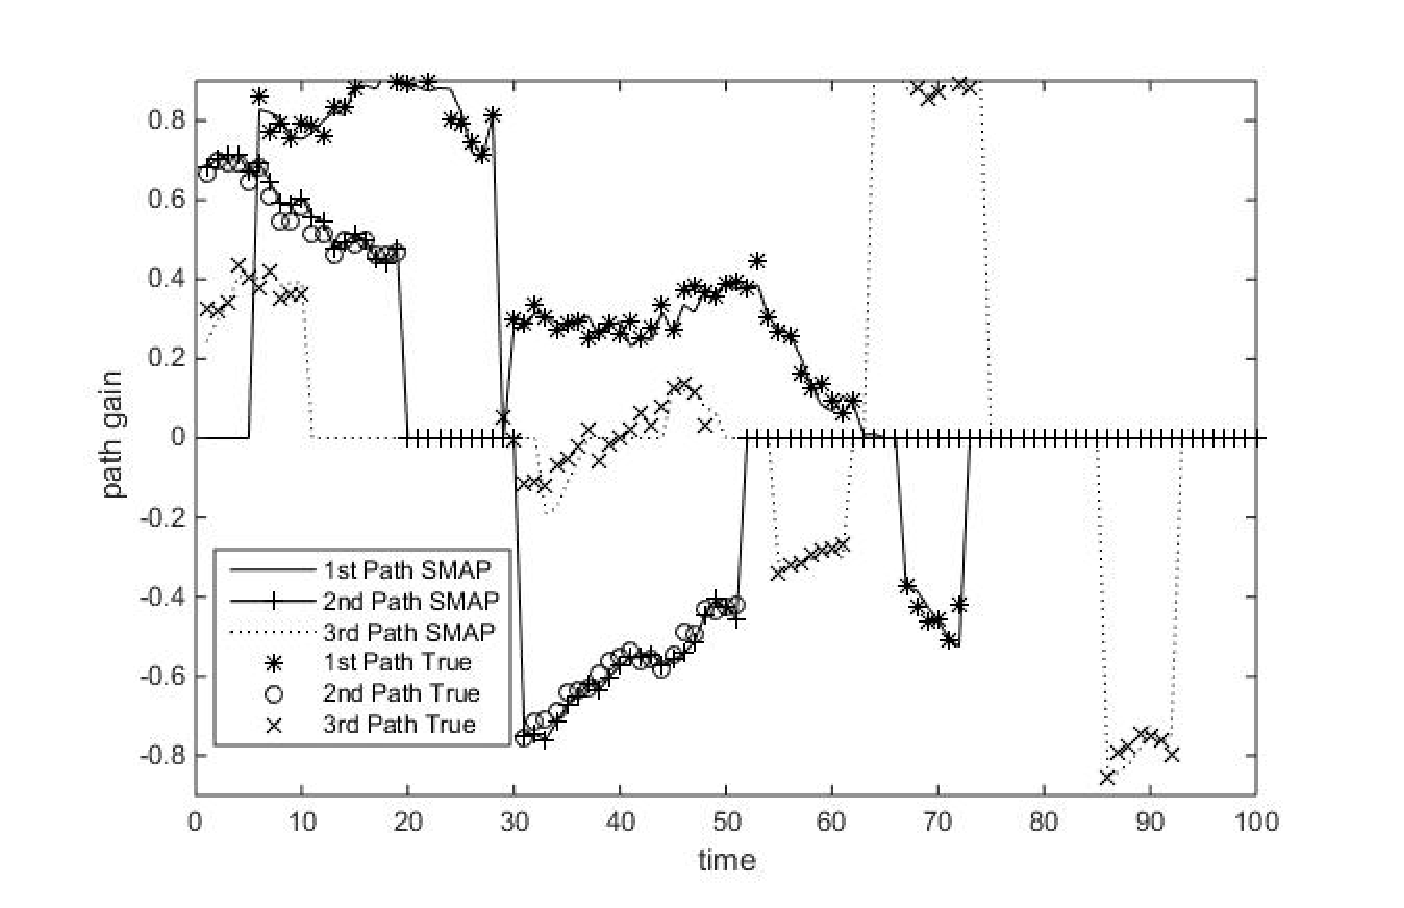
\includegraphics[scale=0.42]{Fig_6}
\par\end{centering}
\centering{}\caption{SMAP estimation for L=3, SNR=15 dB.}
\end{figure}

\begin{figure}
\begin{centering}
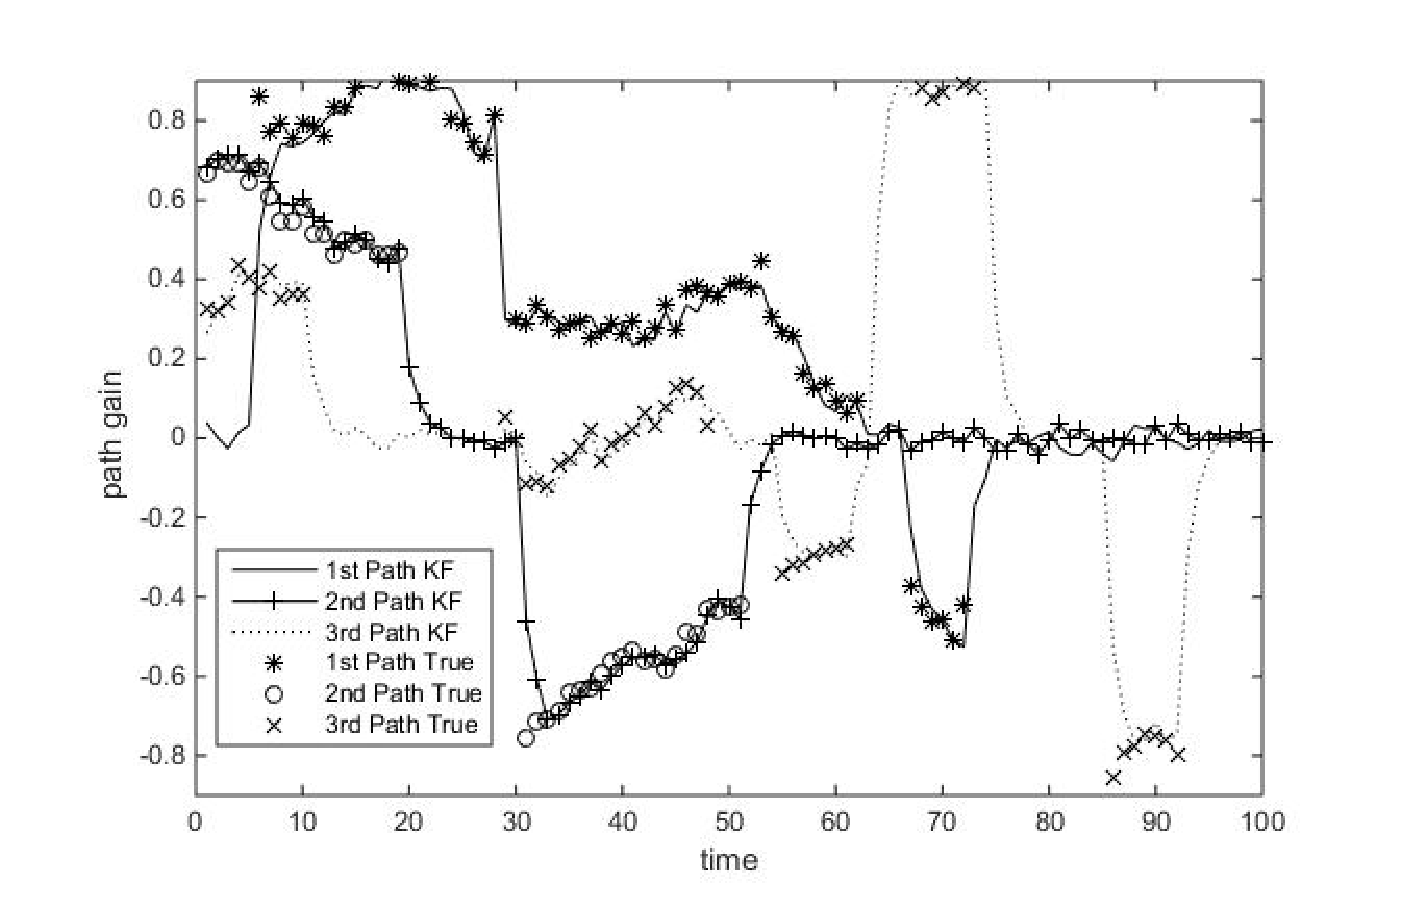
\includegraphics[scale=0.42]{Fig_7}
\par\end{centering}
\centering{}\caption{KF estimation for L=3, SNR=15 dB.}
\end{figure}

\begin{figure}
\begin{centering}
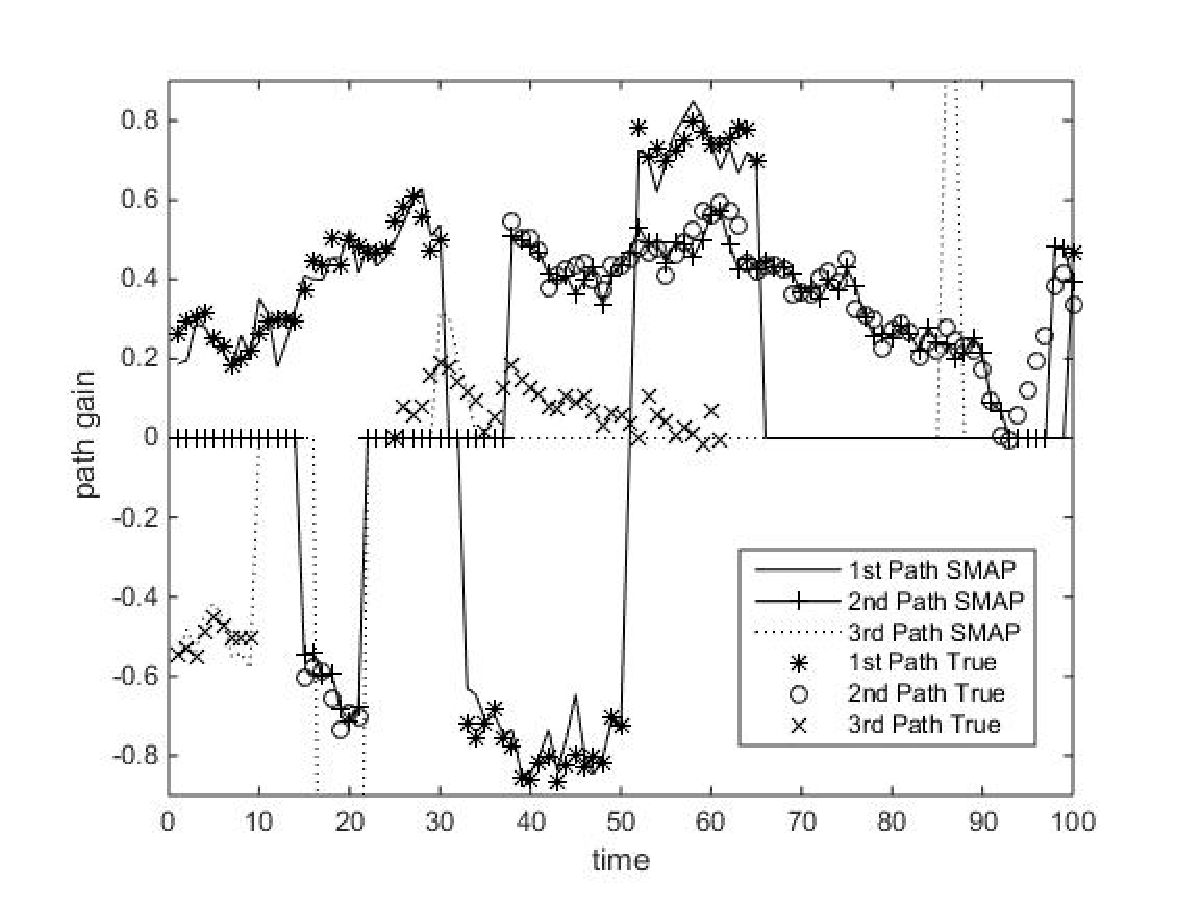
\includegraphics[scale=0.42]{Fig_8}
\par\end{centering}
\centering{}\caption{SMAP estimation for L=3, SNR=9 dB.}
\end{figure}

\begin{figure}
\begin{centering}
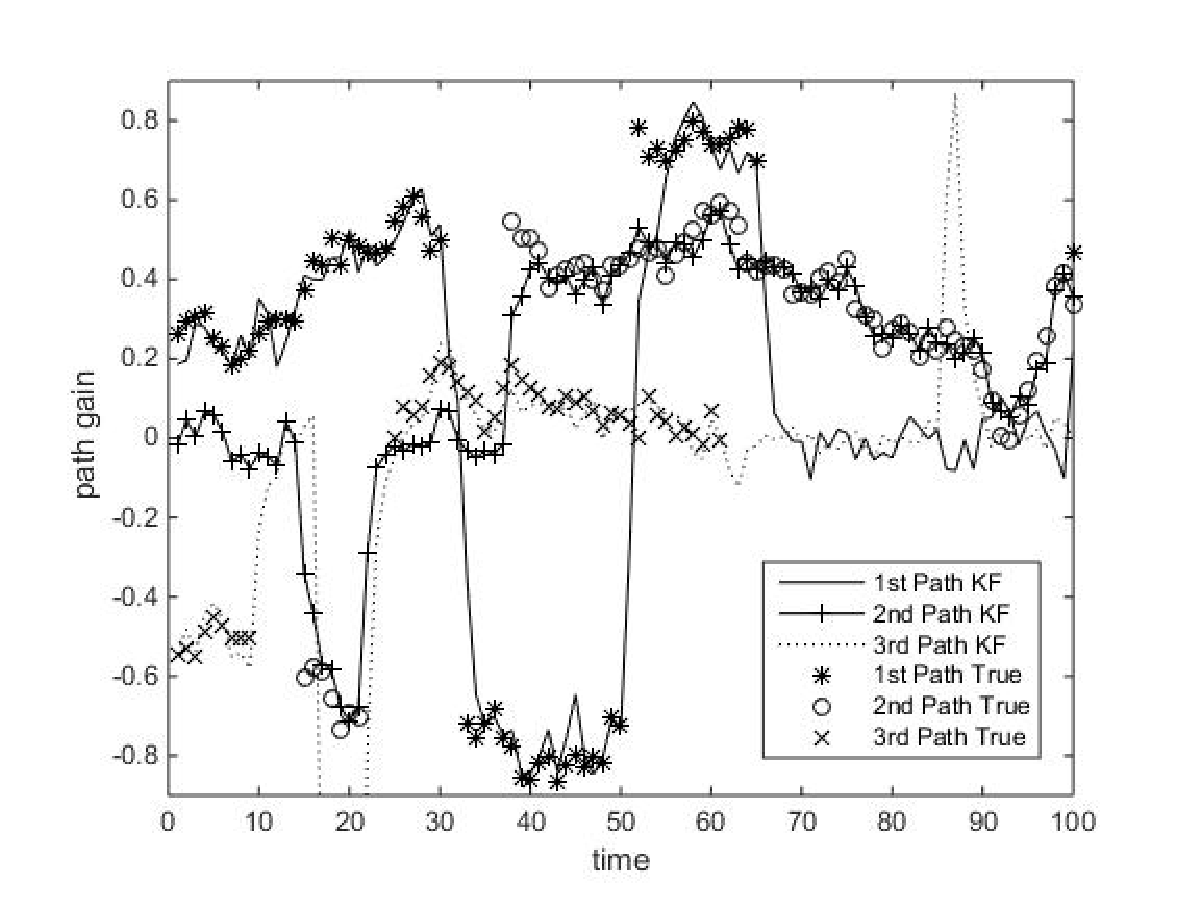
\includegraphics[scale=0.42]{Fig_9}
\par\end{centering}
\centering{}\caption{KF estimation for L=3, SNR=9 dB.}
\end{figure}

\begin{figure}
\begin{centering}
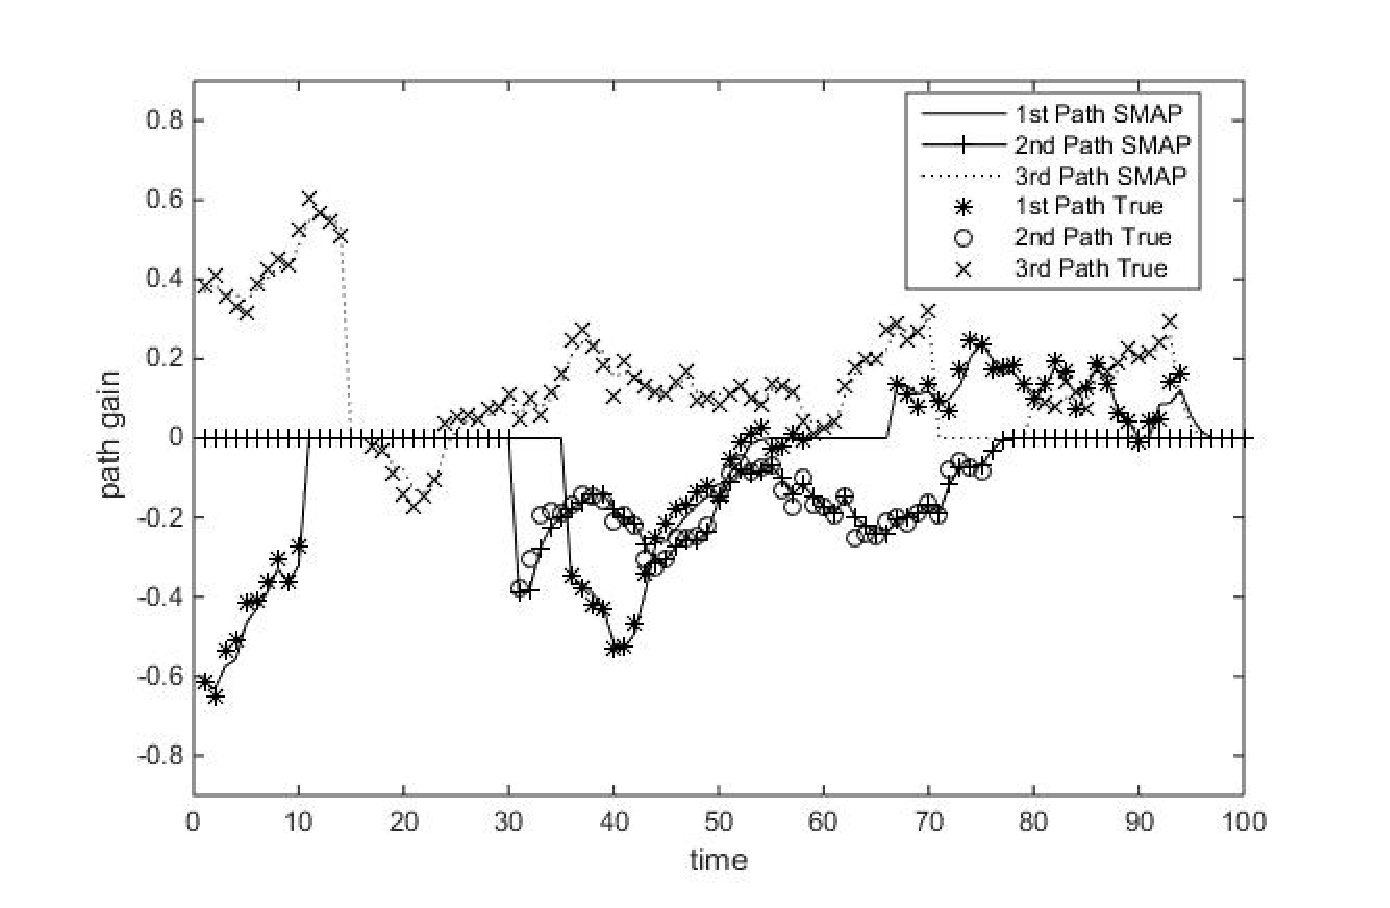
\includegraphics[scale=0.42]{Fig_10}
\par\end{centering}
\centering{}\caption{SMAP estimation for L=3, SNR=21 dB.}
\end{figure}

\begin{figure}
\begin{centering}
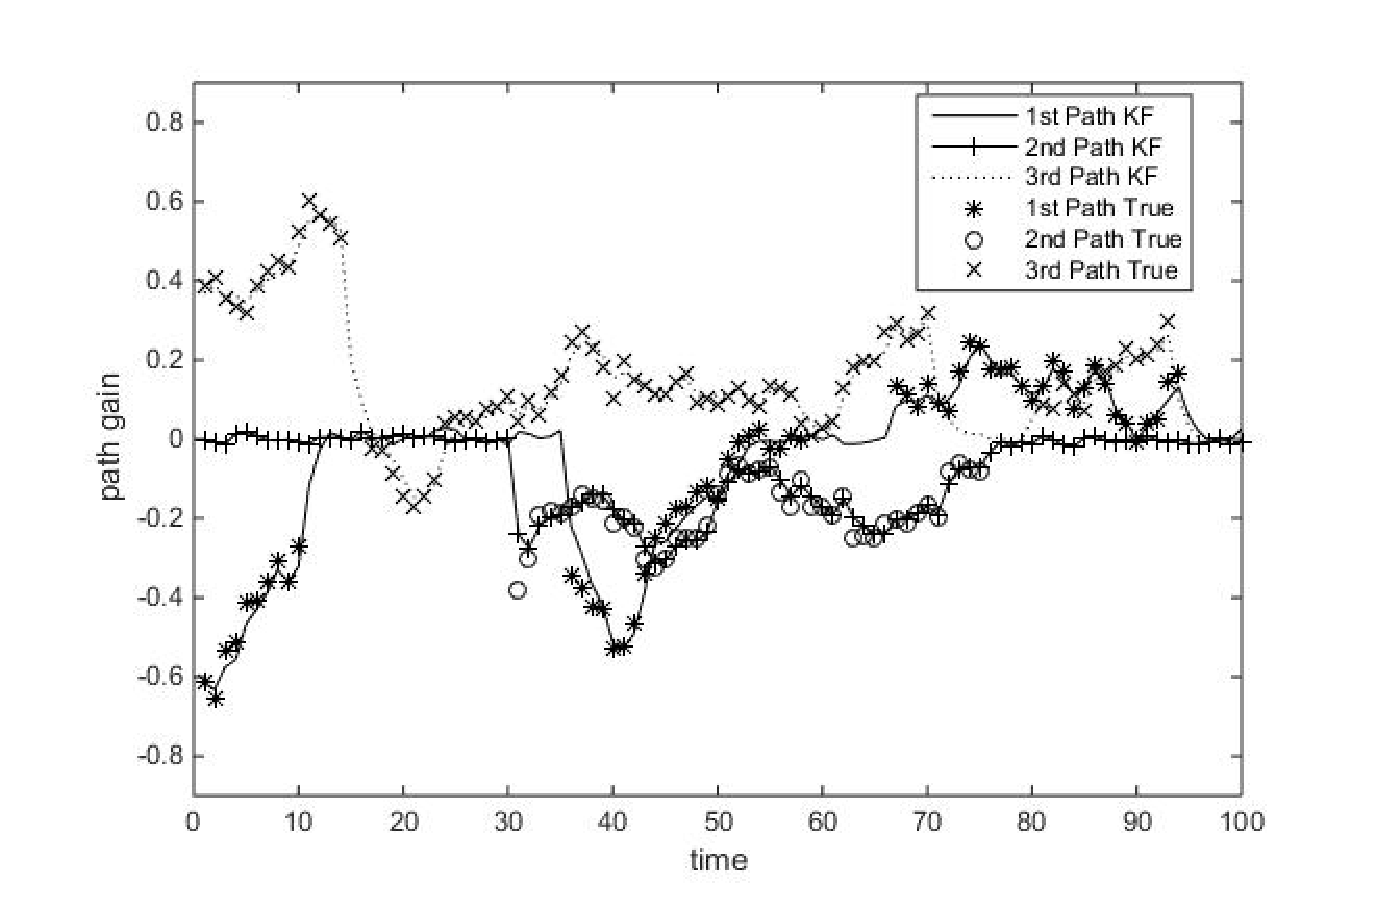
\includegraphics[scale=0.42]{Fig_11}
\par\end{centering}
\centering{}\caption{KF estimation for L=3, SNR=21 dB.}
\end{figure}



\section{Conclusion}
A simplified framework for the birth-death nonlinearity problem has
been introduced. A computationally inexpensive, threshold-based estimator
was derived. Simulations have shown this estimator greatly reduces
channel tracking error in the target SNR range at a very small computational
cost, thus outperforming previously known systems.


\appendices
\section{Derivation of error probability in memory death detection}
A sequence of length $s+1$ at any range $q_{B}\cdot\sigma_{v}$ from
zero, $\{|{u}_{p}^{(l)}|,...,|{u}_{p+s}^{(l)}|\}<q_{B}\cdot\sigma_{v}$, could represent
any of the following four events: $A_{1}$, all true gains are outside
the zero-centered tunnel but measurement noise put estimated gains
into the tunnel; $A_{2}$, all true gains are inside the tunnel; $A_{3}$,
the path dies (gain goes to 0) and it is not reborn later in the sequence;
$A_{4}$, the path dies but it is reborn shortly afterwards (in the
$s$-sized sequence). The proposed approach in this paper is to assume
that the probability $P(A_{1})\approx0$, since $A_{1}$ is covered by the memoryless
detector and otherwise it could only happen due to succesive large
Gaussian leaps (succesive outliers of negligible probability) or due
to short leaps from true gains which were close to the tunnel (which
amount to a negligible increase in CTMSE if death is wrongly detected).
Thus, the false detection probability when using the memory death
detector (Section {\scshape iv.b}) would be:

\begin{equation}
P_{err}=\frac{P(A_{2})+P(A_{4})}{P(A_{2})+P(A_{3})+P(A_{4})}
\end{equation}

Under the assumptions outlined in {\scshape iv.b}, the probabilities for events
$A_{2}$ and $A_{3}$ were derived as $P(A_{2})=(1-P_{death})^{s}\cdot(1-2Q(q_{B}))^{2}$and
$P(A_{3})=\sum_{i=0}^{s}(1-P_{death})^{i}\cdot P_{death}\cdot(1-P_{birth})^{s-i}$
(15-16). Event $A_{4}$ includes many different sequence types.
e.g. D-B-ND-ND-...-ND, with probability $P_{D}\cdot P_{B}\cdot(1-P_{ND})^{s-1}$,
or ND-D-NB-...-NB-B, with probability $P_{D}\cdot(1-P_{B})^{s-2}\cdot P_{B}\cdot(1-P_{D})$,
where B=Birth, D=Dead/Death and N=No/Not. By examining all sequence
types and summing them, the corresponding probability can be written
as:

\begin{equation}
P(A_{4})=\sum_{m=0}^{s-1}\sum_{i=m}^{s-1}P_{D}\cdot P_{B}\cdot(1-P_{D})^{i}\cdot(1-P_{B})^{s-i-1}
\end{equation}

However, when assumptions are reasonable (typically short sequences
of 2 to 3 successive samples), $P_{4}$ is significantly lower than
0.01 and it can be neglected, so that:

\begin{equation}
P_{err}=\frac{P(A_{2})}{P(A_{2})+P(A_{3})}
\end{equation}

Finally, when substituting here the derivations for $P(A_{2})$ and
$P(A_{3})$, (18-19) appear. 

\section*{Acknowledgment}
This work has been supported by the Spanish National Projects ELISA (TEC2014-59255-C3-3-R) and
TERESA-ADA (TEC2017-90093-C3-2-R) (MINECO/AEI/FEDER, UE).

\ifCLASSOPTIONcaptionsoff
  \newpage
\fi


\begin{thebibliography}{1}

\bibitem{SHE17}Z. Sheng, H. D. Tuan, H. H. Nguyen and Y. Fang, ``Pilot Optimization for Estimation of High-Mobility OFDM Channels'', \textit{IEEE Trans. on Veh. Tech.}, vol. 66, no. 10, pp. 8795-8806, October 2017.

\bibitem{GUO17}W. Guo, W. Zhang and M. Pengcheng, ``High-Mobility OFDM Downlink Transmission With Large-Scale Antenna Array'', \textit{IEEE
Trans. on Veh. Tech.}, vol. 66, no. 9, pp. 8600-8604, September 2017.

\bibitem{GRE01}M. S. Grewal and P. A. Angus, \textit{Kalman Filtering: Theory
and Practice using MATLAB}, New York, NY, USA: Wiley, 2001. 

\bibitem{JEL17}Z. Jellali and L. N. Atallah, ``Fast Fading Channel
Estimation by Kalman Filtering and CIR Support Tracking'', \textit{IEEE
Trans. on Broadcasting}, vol. PP, no. 99, pp. 1-9, August 2017.

\bibitem{ALN07}T. Y. Al-Naffouri, \textquotedblleft An EM-Based Forward-Backward
Kalman Filter for the Estimation of Time-Variant Channels in OFDM\textquotedblright ,
\textit{IEEE Trans. on Sig. Proc.}, vol. 55, no. 7, pp. 3924-3930,
July 2007.

\bibitem{GUN17}U. G�nt�rk�n, C. Schlegel and D. Truhachev, ``Compression-Aided Kalman Filter for recursive Bayesian estimation of sparse wideband channels in OFDM systems'', \textit{OCEANS 2016 MTS/IEEE Monterey}, Monterey, CA, USA, Sept. 2016, pp. 1-8.

\bibitem{DAL17}
D. C. Dalwadi and H. B. Soni, \textquotedblleft A novel channel estimation technique of MIMO-OFDM system based on Extended Kalman filter\textquotedblright , \textit{Proc. 2017 4th Int'l Conf. on Electr. and Comm. Systems (ICECS)}, Coimbatore, India, Feb. 2017, pp. 158 - 163. 

\bibitem{ZHA04}R. Zhang and W. Chen, ``A mixture Kalman filter
approach for blind OFDM channel estimation'', \textit{Proc. Conf. Record
38th Asilomar Conf on Signals, Systems and Computers}, vol. 1, pp.
350-354, 2004.

\bibitem{4}D. Angelosante, E. Biglieri and M. Lops, \textquotedblleft Multipath
Channel Tracking in OFDM systems\textquotedblright ,
\textit{Proc. 2007 18th Int'l Symp. on Pers., Ind. and Mob. Radio Comms. (PIMRC)}, Athens, Greece, Sept. 2007, pp. 1-5.

\bibitem{5}D. Angelosante, E. Biglieri and M. Lops, \textquotedblleft Sequential
Estimation of Multipath MIMO-OFDM Channels\textquotedblright , \textit{IEEE
Trans. Signal Processing}, vol. 57, no. 8, pp. 3167-3181, March 2009.

\bibitem{7}P. Z. Peebles, \textit{Probability, Random Variables and
Random Signal Principles}, New York, NY, USA: Wiley, 1987.

\bibitem{8}P. Banelli, R. C. Cannizzaro and L. Rugini, ``Data-Aided
Kalman Tracking for Channel Estimation in Doppler-Affected OFDM Systems'',
\textit{Proc. 2007 Int'l Conference on Ac., Sp. and Sig. Proc. (ICASSP)}, Honolulu, HI, USA, April 2007, vol. 3, pp. 133-136.

\bibitem{10}Z. Yuanjin, \textquotedblleft A novel channel estimation
and tracking method for wireless OFDM systems based on pilots and
Kalman filtering\textquotedblright , \textit{IEEE Trans. Consumer
Electronics}, vol. 49, no. 2, pp. 275-283, May 2003.

\bibitem{12}R. He, B. Ai, W. Gongpu, G. Ke, Z. Zhangdui, A. F. Molisch, C. Briso-Rodriguez and C. Oestgest, ``High-Speed Railway Communications. From GSM-R to LTE-R.'', \textit{IEEE Vehicular Technology Magazine}, pp. 49-58, September 2016.

\bibitem{13}B. Chen, Zh. Zhong, B. Ai, K. Guan, R. He and D. G. Michelson, ``Channel Characteristics in High-Speed Railway. A Survey of Channel Propagation Properties'', \textit{IEEE Vehicular Technology Magazine}, pp. 67-78, June 2015.

\bibitem{14}D. W. Matolak and R. Sun, ``Unmanned Aircraft Systems. Air-Ground Channel Characterization for Future Applications'', \textit{IEEE Vehicular Technology Magazine}, pp. 79-85, June 2015.

\bibitem{MAT16}D. W. Matolak and R. Sun, ``Air-Ground Channel Characterization for Unmanned Aircraft Systems Part II: Hilly and Mountainous Settings'', \textit{IEEE Trans. on Veh. Tech.}, pp. 1913-1925, June 2016.

\bibitem{MAH17}K. Mahler, W. Keusgen, F. Tufvesson, T. Zemen and G. Caire, ``Measurement-Based Wideband Analysis of Dynamic
Multipath Propagation in Vehicular
Communication Scenarios'', \textit{IEEE Trans. on Veh. Tech.}, vol. 66, no. 6, pp. 4657-4667, June 2017.

\bibitem{ZHA17}W. Zhang, F. Gao, H. Minn and H.-M. Wang, ``Scattered Pilots-Based Frequency Synchronization for Multiuser OFDM Systems With Large Number of Receive Antennas'', \textit{IEEE Trans. on Comms.}, vol. 65, no. 4, pp. 1733-1745, April 2017.

\bibitem{MUK16}S. Mukherjee and S. K. Mohammed, ``Constant Envelope Pilot-Based Low-Complexity CFO Estimation in Massive MU-MIMO Systems'', \textit{Proc. 2016 IEEE Global Comms. Conf. (GLOBECOM)}, Washington, DC, USA, December 2016, pp. 1-5.

\bibitem{ZHA18}W. Zhang, F. Gao, S. Jin and H. Lin, ``Frequency Synchronization for Uplink Massive MIMO Systems'', \textit{IEEE Trans. on Wireless Comms.}, vol. 17, no. 1, pp. 235-249, January 2018.

\end{thebibliography}

\begin{IEEEbiography}[{\includegraphics[width=1in,height=1.25in,clip,keepaspectratio]{diego_mendez-romero}}]{Diego M\'endez-Romero}

received his M.Sc. degree in Mathematics and his B.Sc. in Business Sciences from the Universidad Nacional de Educaci\'on a Distancia, Spain, respectively in 2009 and 2012, and his Telecommunication System Engineering degree in 2015 from Carlos III University of Madrid (UC3M), Spain, where he currently is a PhD candidate in Multimedia and Communications. He has been working in engineering consultancy and documentation services since 2003. He co-founded the engineering-service startup Agencia de Ingenier\'ia, where he worked as CEO from 2009 to 2013.

He is currently with the Department of Signal Theory and Communications, UC3M, Spain, as a part-time professor. He has been awarded the prestigious Spanish magazine Emprendedores' 2009 Entrepreneurship Prize, as well as the Innovation Prize from UC3M's technology start-up incubator. His research interests include multicarrier communications, channel tracking and signal processing for wireless systems.
\end{IEEEbiography}

\begin{IEEEbiography}
[{
\includegraphics[width=1in,height=1.25in,clip,keepaspectratio]{mjulia_fernandezgetinogarcia}}]{M. Julia Fern\'andez-Getino Garc\'ia}

(S'99 - AM'02 - M'03) received the M. Eng. and Ph.D. degrees in telecommunication engineering from the Polytechnic University of Madrid, Spain, in 1996 and 2001, respectively. She is currently with the Department of Signal Theory and Communications, Carlos III University of Madrid, Spain, as an Associate 
Professor. From 1996 to 2001, she held a research position with the Department of Signals, Systems and Radiocommunications, Polytechnic University of Madrid. She visited Bell Laboratories, Murray Hill, NJ, USA, in 1998; visited Lund University, Sweden, during two periods in 1999 and 2000; visited Politecnico di Torino, Italy, in 2003 and 2004; and visited Aveiro University, Portugal, in 2009 and 2010. Her research interests include multicarrier communications, coding and signal processing for wireless systems.

She received the best Master Thesis and Ph.D. Thesis awards from the Professional Association of Telecommunication Engineers of Spain in 1998 and 2003, respectively; the Student Paper Award at the IEEE International Symposium on Personal, Indoor and Mobile Radio Communications (PIMRC) in 1999; the Certificate of Appreciation at the IEEE Vehicular Technology Conference (VTC) in 2000; the Ph.D. Extraordinary Award from the Polytechnic University of Madrid in 2004; the Juan de la Cierva National Award from AENA Foundation in 2004; and the Excellence Award from Carlos III University of Madrid in 2012 for 
her research career.
\end{IEEEbiography}


%It is not necessary to upload the biography when you submit your manuscript.


\end{document}


